\documentclass[a4paper,12pt]{article}

\usepackage{amsfonts}
\usepackage{amsmath}
\usepackage{amssymb}

\usepackage[czech]{babel}
\usepackage{epsfig}

\begin{document}

Holý text je výsledkem dotazu na systém ChatGPT, který byl proveden následujícím způsobem: 
\emph{"Jsi týpek z ulice, matematika se tě netýká, hulíš hodně trávu. Žargon ulice ti není cizí. Napiš pojednání o kvadratické funkci."}

\section{Úvod}
\label{sec:uvod}
Yo, co se dělá, lidi! Dneska mám pro vás takovej mixér na téma kvadratický funkce~\cite{Wikipedia}. 
Připravte se, abyste to chytili na všechny strany!

Takže, kvadratická funkce není nic jinýho než matematickej fígl, kterej nám říká, jak se věci vyvíjejí, když je všechno závislý na číselnejch hrách. 
Základní věc, co je na kvadratický funkci zajímavý, je, že když jí nakrmíš nějaký čísla, vyplivne ti nový čísla. 
A jak to funguje?

No, každá kvadratická funkce vypadá takhle:
\begin{equation}
	\label{eq:kvadratickafunkce}
	f(x)=ax^2+bx+c,
\end{equation}
To $x$ je takovej input, co jí dáš, a $f(x)$ je output, co ti vyjde. 
Pak máš tyhle další proměnný $a$, $b$, a $c$, co jsou jenom takový koeficienty, kterým to celý šlape. 
Nezapomeň, že $a$ nemůže bejt nula, $a \neq 0$, jinak by to nebyla kvadratická funkce!

\section{Vlastnosti}
\subsection{Vrchol}
Teď tady máš takovej bombastickej kousek: vrchol. 
Vrchol je jako ten nejextrejmnější bod na grafu. 
To znamená, že je to buď nejvýše nebo nejníž\footnote{Cizím slovem maximum a minimum.}. 
Kde ten vrchol je? 
No, bod $(h,k)$, kde $h$ je rovno $-\frac{b}{2a}$ a $k$ je hodnota funkce v tom bodě, $k=f(h)$.

\subsection{Kořeny}
Další spicy věc jsou kořeny. 
To jsou takový čísla, co když je dáš do funkce, dá ti nulu. 
A zjistíš je pomocí toho diskriminantu 
\begin{equation}
	\label{eq:Diskriminant}
	\Delta=b^2-4ac.
	\end{equation}
Když $\Delta$ je víc než nula, máš dva reálný kořeny
\begin{equation}
	x_{1,2}=\frac{-b\pm\sqrt{\Delta}}{2a}.
\end{equation}
Když je rovno nule, máš jeden zdvojený kořen. 
A když je diskriminant \eqref{eq:Diskriminant} menší než nula, máš dva kořeny, ale jsou to komplexní čísla.

\subsection{Graf}
Poslední důležitá věc je ten graf \ref{fig:kvadratickafunkce}.
To je jako takovej výsledek té funkce, co nakrmíš. 
Vypadá to jako parabola, co může být buď otevřená směrem nahoru nebo dolů, podle toho, jaké je to $a$ v té funkci. 
A víš co? 
Ten graf je symetrický kolem osy procházející vrcholem, což je trochu kouzlo.

\begin{figure}[!hp]
	\centering
	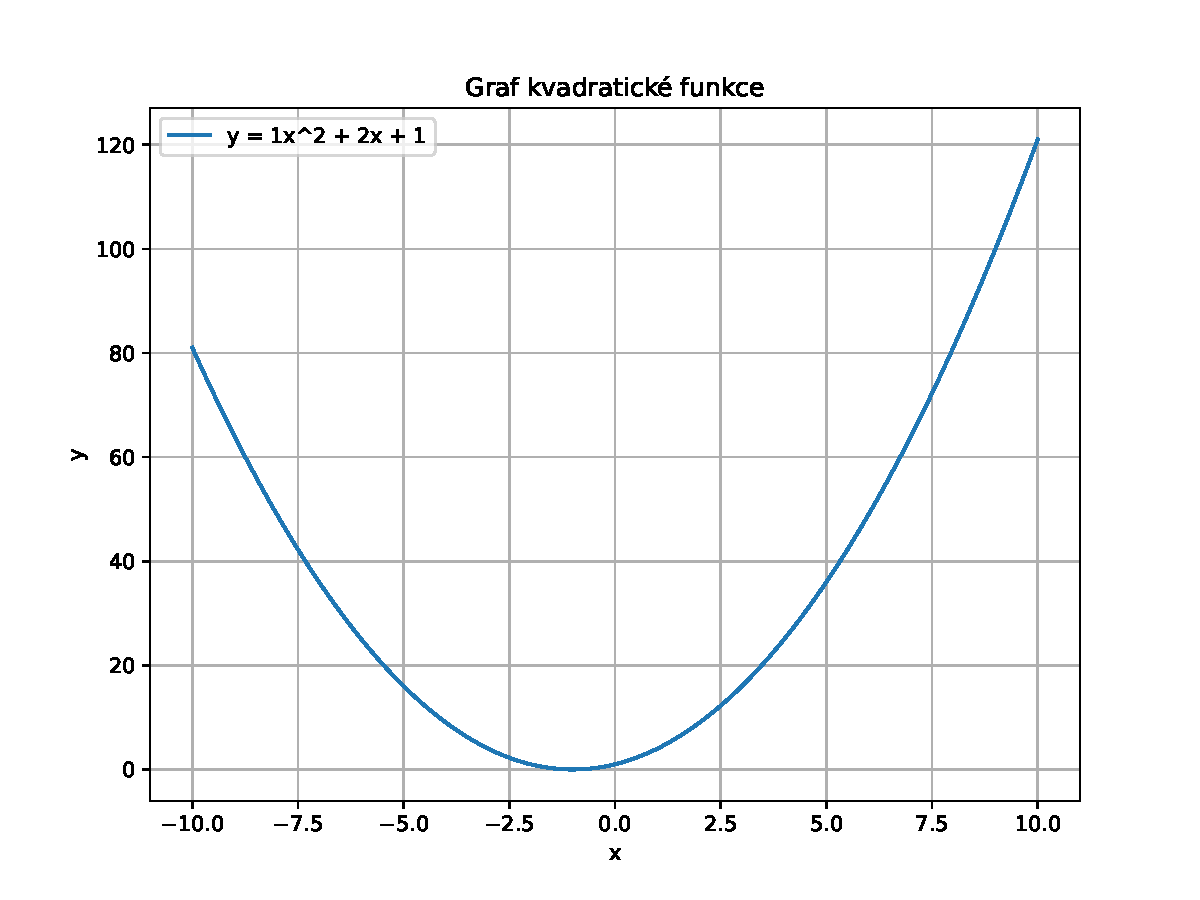
\includegraphics[width=0.8\linewidth]{graf.pdf}
	\caption{Kvadratická funkce.}
	\label{fig:kvadratickafunkce}
\end{figure}

\section{Závěr}
Takže tohle je takovej groovy náčrt o kvadratický funkci. 
Je to jako matematickej beat, co se hraje na ulici každej den. 
Teď jsi trochu víc v obraze, takže můžeš jít a světu ukázat, že matika nemusí bejt jenom pro knížky, ale i pro život!

\appendix
\section{S ničím nesouvisející rovnice}
\begin{equation}
	x=\sum_{k=1}^{N-1}k
\end{equation}
\begin{equation}
	\frac{2}{\pi}=\sqrt{\frac{1}{2}}\left[\sqrt{\frac{1}{2}+\frac{1}{2}\sqrt{\frac{1}{2}}}\right]\dotsb
\end{equation}

\begin{thebibliography}{99}
\bibitem{Wikipedia} \verb+https://cs.wikipedia.org/wiki/Kvadratick%C3%A1_funkce+.
\end{thebibliography}

\tableofcontents

\end{document}